%!TEX root = ../../IF.tex
\definecolor{verde}{HTML}{00FF00}
\newcommand*\Terminal[5]{
\begin{tikzpicture}
\tikzset{mystyle/.style={right, text ragged, rounded corners,fill={#3}, inner sep=1ex,text width = {#1}}}
{\fontsize{#2}{2} \selectfont%
\node[mystyle]{\color{#4}\textbf{#5}};
}%
\end{tikzpicture}
}
% Exemplo de definicao de um novo estilo do pacote listings:
%----------------------------------------------------------------------------------
\lstdefinestyle{lista}{%
    literate=
    {á}{{\'a}}1 {é}{{\'e}}1 {í}{{\'i}}1 {ó}{{\'o}}1 {ú}{{\'u}}1 {ù}{{\`u}}1
    {Á}{{\'A}}1 {É}{{\'E}}1 {Í}{{\'I}}1 {Ó}{{\'O}}1 {Ú}{{\'U}}1
    {à}{{\`a}}1 {è}{{\'e}}1 {ì}{{\`i}}1 {ò}{{\`o}}1 {ò}{{\`o}}1
    {À}{{\`A}}1 {È}{{\'E}}1 {Ì}{{\`I}}1 {Ò}{{\`O}}1 {Ò}{{\`O}}1
    {ä}{{\"a}}1 {ë}{{\"e}}1 {ï}{{\"i}}1 {ö}{{\"o}}1 {ü}{{\"u}}1
    {Ä}{{\"A}}1 {Ë}{{\"E}}1 {Ï}{{\"I}}1 {Ö}{{\"O}}1 {Ü}{{\"U}}1
    {â}{{\^a}}1 {ê}{{\^e}}1 {î}{{\^i}}1 {ô}{{\^o}}1 {û}{{\^u}}1
    {Â}{{\^A}}1 {Ê}{{\^E}}1 {Î}{{\^I}}1 {Ô}{{\^O}}1 {Û}{{\^U}}1
    {ã}{{\~a}}1 {Ã}{{\~A}}1 {õ}{{\~o}}1 {Õ}{{\˜O}}1    
    {œ}{{\oe}}1 {Œ}{{\OE}}1 {æ}{{\ae}}1 {Æ}{{\AE}}1 {ß}{{\ss}}1
    {ç}{{\c c}}1 {Ç}{{\c C}}1 {ø}{{\o}}1 {å}{{\r a}}1 {Å}{{\r A}}1
    {€}{{\EUR}}1 {£}{{\pounds}}1,
    % inputencoding=latin1,
    upquote=true,
    % extendchars=true,
    breaklines=true,
    breakautoindent=true,
    linewidth=\linewidth,
    % numbers=left,
    numberstyle=\footnotesize,
    numbersep=1em,
    % xleftmargin=1em,
    framextopmargin=5pt,
    framexbottommargin=5pt,
    showspaces=false,
    showtabs=false,
    showstringspaces=false,
    % frame=l,
    frameround=tttt,
    aboveskip=20pt,
    belowskip=20pt,
    tabsize=4,
    basicstyle=\ttfamily\small,
    backgroundcolor=\color{gray!5},
    commentstyle=\color{Comments}\slshape,
    stringstyle=\color{Strings},
    morecomment=[s][\color{Strings}]{"""}{"""},
    morecomment=[s][\color{Strings}]{'''}{'''},
    keywordstyle={\color{black}\bfseries},
    keywordstyle={[2]\color{Decorators}\slshape},
    rulecolor=\color{red}
}
%==================================================================================
\chapter{Introdução}
%==================================================================================
\label{capitulo1}

A classe \LaTeX\ \texttt{if-ufg.cls}\footnote{\copyright\ 2015 Alexandre Barbosa de Almeida (abatriuno@hotmail.com).} foi desenvolvida para auxiliar, com base nas normas da ABNT (Associação Brasileira de Normas Técnicas), na formatação de trabalhos acadêmicos do Instituto de Física da Universidade Federal de Goiás. É possível formatar trabalhos de conclusão de curso (TCC), monografia, qualificação de mestrado, dissertação de mestrado, qualificação de doutorado e \mbox{tese de doutorado.}

\LaTeX\ é uma linguagem de marcação muito utilizada para a diagramação de textos científicos e matemáticos, devido à sua alta qualidade em representar tipografias e símbolos em equações, porém vai muito além disto! Caso ainda não conheça ou saiba pouco sobre \LaTeX, este documento \citeonline{latex_intro:2015} irá ensinar os princípios básicos de como usar este incrível sistema de preparação de documentos. Mais informações podem ser obtidas no site oficial \citeonline{latex:2015}.

O modelo que esta classe adota segue o do Instituto de Informática (UFG) escrito e mantido pelo Prof. Dr. Humberto Longo. Tecnicamente,
esta classe se baseia na classe \texttt{report} e adota o estilo de citacação \texttt{abntex2cite}, sendo que atualmente ambas estão inclusas em toda instalação padrão do \citeonline{texlive:2015}. A classe \texttt{if-ufg.cls} foi designada a fim de atender as normas principais da ABNT no que diz respeito à formatação de trabalhos acadêmicos, contudo ela se difere da classe \texttt{abntex2} mantida pelo grupo \citeonline{abntex2:2015}, que é muito mais completa e busca seguir todas as normas em vigor, sem grandes alterações.

O importante a ser dito é que cada faculdade ou universidade é livre para seguir ou não as normas da ABNT, isto não se faz obrigatório. O que normalmente ocorre é que as faculdades adotam modelos próprios \emph{baseados} na ABNT, com ligeiras modificações, como é o caso desta classe. Outras faculdades acham ridículas as normas da ABNT (com certa razão), e estabelecem as suas próprias. Portanto, sinta-se livre para:

\begin{itemize}
\item Executar o programa como você desejar, para qualquer propósito (liberdade 0);
\item Estudar como o programa funciona, e adaptá-lo às suas necessidades (liberdade 1);
\item Redistribuir cópias de modo que você possa ajudar ao próximo (liberdade 2);
\item Distribuir cópias de suas versões modificadas a outros (liberdade 3). Desta forma, você pode dar a toda comunidade a chance de se beneficiar com as suas mudanças.
\end{itemize}

Esta classe também é muito útil para orientadores e membros de banca, veja que foi implementado um pequeno truque na Seção \ref{refbibliografica} para ajudar na revisão bibliográfica. Aproveitem!

%==================================================================================
\section{Valor Institucional}
%==================================================================================

É costume que os trabalhos acadêmicos sejam copiados ou xerocados para os mais diversos fins. Geralmente, a informação mais marcante relativa à instituição onde o trabalho foi produzido é o logotipo estampado na página de capa, e no restante do trabalho essa informação se ``perde''.

Esta classe traz em seu \emph{layout} o logotipo e o nome da instituição em quase todas as páginas, de um modo a valorizar a instituição onde o trabalho foi concluído, assim, se o trabalho for xerocado, ou distribuído, seja em parte ou no todo, haverá um identificador da instituição de modo a conferir certa autenticidade de origem ao material em questão.

%==================================================================================
\section{Requisitos de Software}
%==================================================================================

Para fins de atualizações e manter a compatibilidade da classe com os pacotes utilizados, recomenda-se instalar a versão completa do \TeX Live 2014 (ou posterior) e, de perferência, que se utilize alguma distribuição de Linux ou Mac OS X. Para fins didáticos, as instruções a seguir presume que o usuário utilize o sistema operacional Ubuntu, no entanto, usuários de \LaTeX\ acostumados com os sistemas Windows e Mac OS X poderão facilmente concluir a instalação dos requisitos.

Esta classe foi desenvolvida em um Mac OS X Yosemite, utilizando o editor Sublime Text 3 (\emph{plugin} LaTeXTools), com a versão completa do \TeX\ Live 2014 baixada de \citeonline{mactex:2015} e compilada com o \Verb+pdflatex+, versão 2.6-1.40.15.

%==================================================================================
\subsection{Instalando o \TeX\ Live 2014}
%==================================================================================

Recomenda-se excluir qualquer versão anterior para evitar eventuais problemas. Baixe a imagem \textbf{.iso}\footnote{Disponível em: <http://repositorios.cpai.unb.br/ctan/systems/texlive/Images>. Acessado em: 19 abr. 2015.} do \TeX\ Live 2014 conforme mostrado na Figura \ref{texlive2014}.

Ao descompactar o arquivo \textbf{.iso}, será criada uma pasta denominada \mbox{\drawtikzfolder\  \texttt{texlive2014}} com os arquivos extraídos. Provavelmente será necessário alterar as permissões dos conteúdos presentes na pasta, então abra um terminal no diretório em que se localiza a pasta recém criada e digite os seguintes comandos:\vspace{10pt}

\noindent
\Terminal{0.96\textwidth}{10pt}{black!70}{verde}{\ttfamily \$ sudo chmod -R 777 texlive2014 \\[5pt] \ttfamily \$ cd texlive2014 \\[5pt] \ttfamily \$ ./install-tl }

\vspace*{5pt}
\noindent
Siga as instruções e termine a instalação. Note que serão instalados todos os pacotes presentes no \TeX\ Live 2014, ocupando em torno de 2.5 Gb.

Agora é preciso colocar a nova instalação do \TeX Live 2014 no PATH do sistema para que possa ser encontrado pelos compiladores, então adicione a seguinte linha:

\begin{center}
{\ttfamily /usr/local/texlive/2013/bin/x86\_64-linux} 
\end{center}

\noindent
ao arquivo \drawtikzfolder\ {\ttfamily /etc/environment}:
\vspace*{10pt}

\noindent
\Terminal{0.96\textwidth}{10pt}{black!70}{verde}{\ttfamily \$ sudo gedit /etc/environment}

\vspace*{5pt}
\noindent
O arquivo \drawtikzfolder\ {\ttfamily /etc/environment} deve ficar algo parecido com isto:

\vspace*{10pt}
\begin{center}
PATH=``/usr/local/texlive/2014/bin/x86\_64-linux:/usr/local/sbin:-/usr/local/bin:/usr/sbin:/usr/bin:/sbin:/bin:/usr/games:-/usr/local/games''
\end{center}

\begin{figure}[!ht]
\centering
\caption{Faça o download do arquivo \textbf{texlive2014.iso}.}\label{texlive2014}
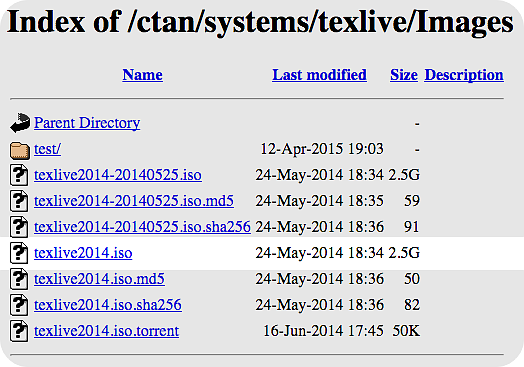
\includegraphics[width=0.7\textwidth]{./figuras/texlive2014.png}
\fonte{autor.}
\end{figure}

%==================================================================================
\section{Estrutura dos Trabalhos Acadêmicos}
%==================================================================================

De acordo com a norma \citeonline{NBR14724:2011}, os trabalhos acadêmicos estruturam-se da seguinte maneira: elementos pré-textuais, elementos textuais e elementos pós-textuais.

%==================================================================================
\subsection{Elementos pré-textuais}
%==================================================================================

São as páginas com informações que antecedem o texto principal do trabalho, são elas: capa (obrigatório), ficha catalográfica (opcional), folha de rosto (obrigatório), errata (opcional), folha de aprovação (obrigatório), dedicatória (opcional), agradecimentos (opcional), epígrafe (opcional), resumo em língua vernácula com palavras-chave (obrigatório), resumo em língua estrangeira com palavras-chave (obrigatório), lista de ilustrações (opcional), lista de tabelas (opcional), lista de abreviações ou siglas (opcional), lista de símbolos (opcional), ou quaisquer outros tipos de lista que se deseja criar, como lista de algoritmos e lista de códigos de programas e, por fim, sumário (obrigatório).

%==================================================================================
\subsection{Elementos textuais}
%==================================================================================

Consiste no texto principal, compreende a introdução, o desenvolvimento e a conclusão do trabalho.

%==================================================================================
\subsection{Elementos pós-textuais}
%==================================================================================

Os pós-textuais compreendem as referências bibliográficas (obrigatório), o glossário (obrigatório), o apêndice (opcional), o anexo (opcional) e o índice (opcional) que completam o trabalho principal.

%==================================================================================
\section{\emph{Workspace}}
%==================================================================================

Para uma melhor organização da estrutura de diretórios na qual você fará o seu trabalho acadêmico, vamos utilizar o conceito de \emph{workspace}. Um \emph{workspace} pode ser entendido como uma estrutura de diretórios onde será desenvolvido o seu projeto, ajuda a manter o trabalho coeso, organizado, bem estruturado e de fácil acesso e manutenção.

\bgroup
\usetikzlibrary{trees}
\tikzstyle{every node}=[draw=black, thick, rounded corners, drop shadow, text centered, anchor=west, fill=gray!15]
\tikzstyle{subfolder1}=[text=white,draw={rgb:red,255;green,134;blue,98},fill={rgb:red,255;green,134;blue,98}]
\tikzstyle{subfolder2}=[draw=yellow,fill=yellow!40]
\tikzstyle{subfolder3}=[draw=green,fill=green!20]
\tikzstyle{capitulo_tex}=[draw=blue,fill=blue!20]
\tikzstyle{raiz}=[rectangle, draw=black, thick, rounded corners, fill=black, drop shadow,
        text centered, anchor=north, text=white, text width=5cm]

{\fontsize{8pt}{1.5} \selectfont
\begin{figure}[!ht]
\centering
\caption{Estrutura de um \emph{workspace}.}
\vspace{10pt}
\resizebox{!}{1.15\textwidth}{
\begin{tikzpicture}[%
  grow via three points={one child at (0.5,-0.7) and
  two children at (0.5,-0.7) and (0.5,-1.4)},
  edge from parent path={(\tikzparentnode.south) |- (\tikzchildnode.west)}]
  \node [raiz]{\large \textbf{WORKSPACE}}
  child [missing]{}  
  child { node {IF.tex}}
  child { node {if-ufg.cls}}  
  child { node {Makefile}}
  child [missing]{}    
  child { node [subfolder1] {\textbf{pre\_textuais}}
      child { node {pre\_config.tex}}  
      child { node {agradecimentos.tex}}
      child { node {copyright.tex}}
      child { node {dedicatoria.tex}}
      child { node {epigrafe.tex}}
      child { node {resumo.tex}}
      child [missing]{}       
  }
  child [missing]{}  
  child [missing]{}
  child [missing]{}
  child [missing]{}
  child [missing]{}
  child [missing]{} 
  child { node [subfolder1] {\textbf{textuais}}
      child { node {textuais\_config.tex}}
        child { node [subfolder2] {\textbf{capitulo1}}
          child { node {capitulo1.tex}}
          child { node [subfolder3] {\textbf{figuras}}
            child { node {figura1.png}}        
          }        
        }
        child [missing]{} 
        child [missing]{} 
        child [missing]{}         
        child { node [subfolder2] {\textbf{capitulo2}}
          child { node {capitulo2.tex}}
          child { node [subfolder3] {\textbf{figuras}}
            child { node {figura1.png}}        
          }        
        }        
        child [missing]{}               
  }
  child [missing]{}  
  child [missing]{}
  child [missing]{}
  child [missing]{}
  child [missing]{}
  child [missing]{}                                      
  child [missing]{}
  child [missing]{}
  child [missing]{}
  child { node [subfolder1] {\textbf{pos\_textuais}}
      child { node {pos\_config.tex}}
      child { node [subfolder2] {bibliografia}
        child { node {bibliografia.tex}}
      }
      child [missing]{}      
      child { node [subfolder2] {apendices}
        child { node {apendices.tex}}
      }    
      child [missing]{}      
      child { node [subfolder2] {anexos}
        child { node {anexos.tex}}
      }                   
  }       
  ;
\end{tikzpicture}
}
\vspace*{5pt}
\fonte{autor.}
\label{fig:workspace}
\end{figure}
}
\egroup

Neste nosso exemplo de \emph{workspace}, no diretório raiz têm-se os arquivos \texttt{IF.tex} (principal), \texttt{if-ufg.cls} (classe) e \texttt{Makefile} (executável), e os diretórios \drawtikzfolder\ \texttt{pre\_textuais}, \mbox{\drawtikzfolder\ \texttt{textuais}} e \drawtikzfolder\ \texttt{pos\_textuais}. 

No diretório \drawtikzfolder\ \texttt{pre\_textuais} estão os arquivos que constituem os elementos pré-textuais do trabalho, além do arquivo de configuração \texttt{pre\_config.tex}, que será necessário abrir e editar para inserir as suas informações.

No diretório \drawtikzfolder\ \texttt{textuais}, estão os capítulos que constituem o seu trabalho. Abra e edite o arquivo de configuração \texttt{textuais\_config}. Faça o mesmo para o diretório \mbox{\drawtikzfolder\ \texttt{pos\_textuais}}, onde se encontram os arquivos de \texttt{pos\_config.tex} e os diretórios \mbox{\drawtikzfolder\ \texttt{bibliografia}}, \drawtikzfolder\ \texttt{apendices} e \drawtikzfolder\ \texttt{anexos}.

\vspace{20pt}
\noindent
\textcolor{red}{\uline{ATENÇÃO}}: Fique atento para sempre estar atualizando os arquivos de configurações \texttt{pre\_config.tex}, \texttt{textuais\_config.tex} e \texttt{pos\_config.tex}. Não altere a ordem em que os comandos são chamados nos arquivos, a menos que você saiba o que \mbox{esteja fazendo.}
\vspace{20pt}

Para cada novo capítulo do seu trabalho, crie uma pasta dentro do diretório \mbox{\drawtikzfolder\ \texttt{textuais}}, seguindo a lógica do \emph{workspace} e atualize o arquivo \texttt{textuais\_config.tex}. Veja o exemplo abaixo da Fig.\ref{fig:workspace}.

%==================================================================================
\section{Makefile}
%==================================================================================

Atualmente, o arquivo \texttt{Makefile} é compatível com os sistemas operacionais Linux e Mac OS X:

\importarcodigo{}{Arquivo Makefile.}{Makefile}

Para quem não conhece o uso de um arquivo \texttt{Makefile}, ele contém um conjunto de instruções para compilar o projeto adequamente. Ao utilizar o \texttt{Makefile}, você não precisa mais compilar o seu documento \LaTeX\ do jeito tradicional, provavelmente apertando um botão dentro do seu editor de texto para projetos \LaTeX\ (ex.: Kile, TexMaker, TexShop, etc.). Basta abrir um terminal no diretório em que se encontra o arquivo \texttt{IF.tex} e digitar:\vspace{15pt}

\noindent
\Terminal{0.96\textwidth}{10pt}{black!70}{verde}{\ttfamily \$ make}

\vspace{20pt}
\noindent
\textcolor{red}{\uline{IMPORTANTE}}: Muito provavelmente você vai escolher um nome diferente de \textbf{IF.tex} para escrever o seu trabalho. Caso isto ocorra, substitua (na linha 1 do \texttt{Makefile}) o nome \textbf{IF} pelo novo nome do seu trabalho (sem a extensão \emph{.tex}): \Verb+ARQUIVO=novo_nome+.
\vspace{20pt}

\noindent
\textcolor{red}{\uline{ATENÇÃO}}: Não utilize espaços ou caracteres especiais nos nomes dos diretórios, arquivos e figuras dentro do \emph{workspace}. EVITE AO MÁXIMO esta prática, uma hora ou outra vai dar problema.
\vspace{20pt}

\noindent
\textcolor{red}{\uline{RECOMENDAÇÃO}}: Sempre que puder, prefira utilizar o \texttt{Makefile} para construir os seus projetos. Na maioria das vezes ele contém instruções específicas feitas especialmente para executar o projeto ao qual está associado.
\vspace{20pt}

%==================================================================================
\section{Bugs Conhecidos}
%==================================================================================

\begin{itemize}
\item \textbf{Referência bibliográfica dentro de} \Verb+\caption{\cite{bibkey}}+ \textbf{em figuras ou tabelas}: quando isto acontece, pode ocorrer que a referência da página na \emph{lista de figuras} seja gerada de forma errada. 

\begin{itemize}
\item \textbf{SOLUÇÃO:} antes de mandar compilar novamente o projeto, é necessário excluir o arquivo de extensão \textbf{.toc} (\emph{table of contents}). Exclua este arquivo e compile novamente. 
\end{itemize}

O uso do \texttt{Makefile} resolve este problema automaticamente.
\end{itemize}

%==================================================================================
\section{Licença de Uso}
%==================================================================================

Esta classe está disponível sob a licença da \citeonline{gnulicense:2015}. Caso faça alguma alteração na classe, renomeie o arquivo \texttt{if-ufg.cls} com um nome diferente a fim de garantir a originalidade, integridade e continuidade deste trabalho.
